   \frame{
  \frametitle {Create a docker image for FastQC tool}
\vspace{0.4cm}
   \centerline{\color{NavyBlue} \textbf{\emph{FastQC in nutshell}}}\vspace{0.4cm}
   \begin{itemize}
   \item It is  quality control tool for high throughput sequence data;\vspace{0.2cm}
   \item It is written in Java;\vspace{0.2cm}
   \item It is main functions are:\vspace{0.1cm}
   \begin{itemize}
   \item Import of data from BAM, SAM or FastQ files (any variant);\vspace{0.1cm}
   \item Providing a quick overview to tell you in which areas there may be problems;\vspace{0.1cm}
   \item Summary graphs and tables to quickly assess your data;\vspace{0.1cm}
   \item Export of results to an HTML based permanent report;\vspace{0.1cm}
   \item Offline operation to allow automated generation of reports without running the interactive application.
   \end{itemize} 
   \end{itemize}     	
   \begin{center}
  			
\includegraphics[width=0.15\columnwidth]{./Figure/QC}
  		\end{center} 
  }
  
 \frame{
  \frametitle {Create a docker image for FastQC tool}
   \centerline{\color{NavyBlue} \textbf{\emph{How to create FastQC image}}}\vspace{0.4cm}
  \begin{itemize}
  \item Download and update a basic image (use Fedora);\vspace{0.2cm}
  \item Download and install \textbf{\color{NavyBlue}Oracle Java} on the download image;\vspace{0.2cm}
  \item Download and install  \textbf{\color{NavyBlue}unzip} on the download image;\vspace{0.2cm}
  \item Download and install  \textbf{\color{NavyBlue}perl} on the download image;\vspace{0.2cm}
  \item Download and install  \textbf{\color{NavyBlue}FastQC} on the download image;\vspace{0.2cm}
  \item Run the embedded FastQC on fastq data.
\end{itemize}     
  }

\frame{
  \frametitle {Download and update a basic image}
  \begin{itemize}
  	\item Download Fedora; 
  	          	\begin{center}
  			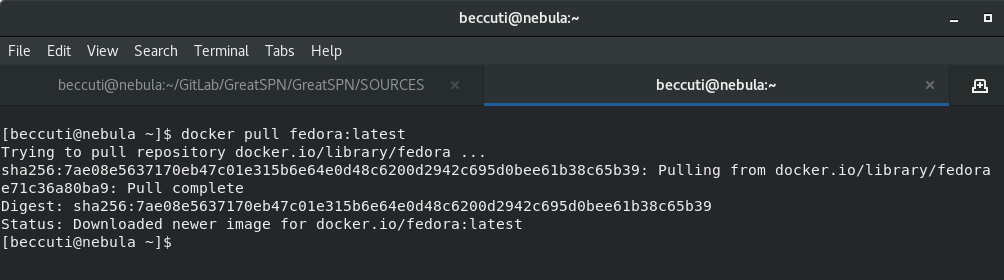
\includegraphics[width=0.95\columnwidth]{./Figure/pullFedora}
  		\end{center}	
  		
  	 \end{itemize}	
  		}
  		
  		
 \frame{
  \frametitle {Download and update a basic image}
  \begin{itemize} 		
  	\item Create a new tag from Fedora image.
          	\begin{center}
  			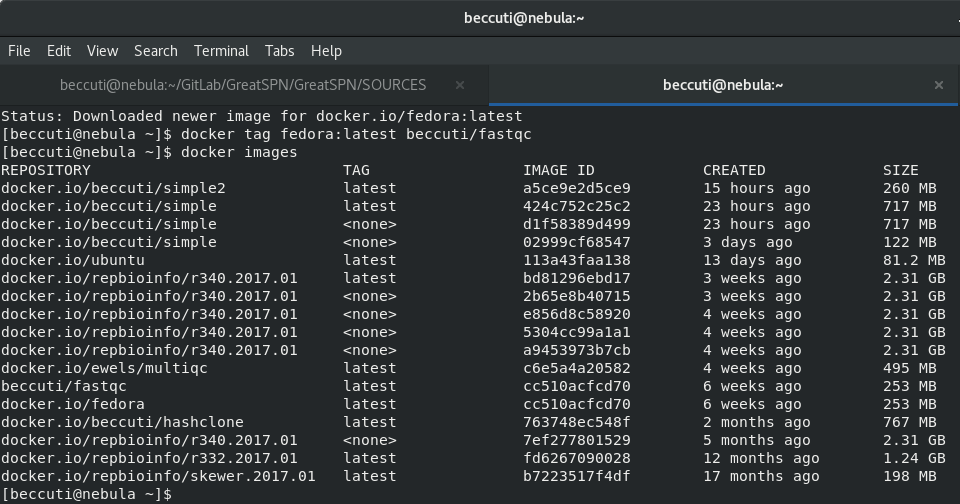
\includegraphics[width=0.95\columnwidth]{./Figure/tagFastQC}
  			\end{center}	
 \end{itemize}
} 
  	 
 \frame{
  \frametitle {Download and update a basic image}
  \begin{itemize} 		
  	\item Update Fedora using \emph{\color{PineGreen} dnf update};
          	\begin{center}
  			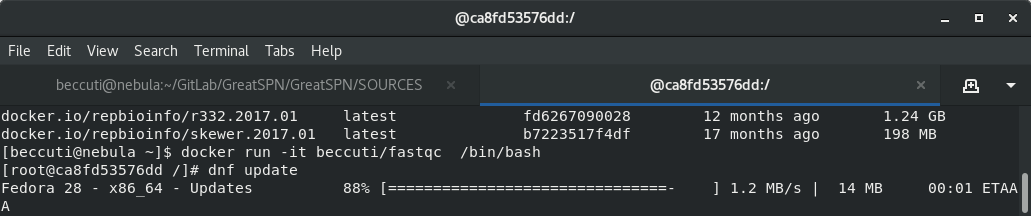
\includegraphics[width=0.95\columnwidth]{./Figure/updateFedora}
  			\end{center}	
   \item  Commit the updated image.
   		    \begin{center}
  			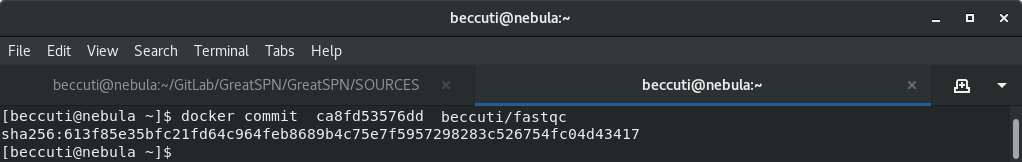
\includegraphics[width=0.95\columnwidth]{./Figure/commitFedora}
  			\end{center}	
 \end{itemize}
} 
  	\frame{
  \frametitle {Download and install Oracle Java}
  \begin{itemize} 		
  	\item Download \textbf{\color{NavyBlue}Java RE ORACLE} (\url{http://www.oracle.com});\vspace{0.2cm}
  	\item Install  \textbf{\color{NavyBlue}Java RE ORACLE}
          	\begin{center}
  			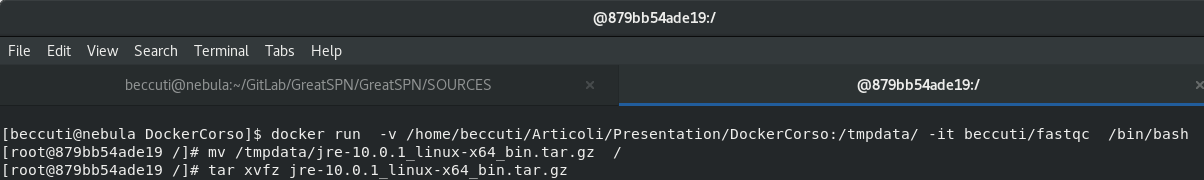
\includegraphics[width=0.95\columnwidth]{./Figure/javaFedora}\vspace{0.2cm}
  			\end{center}	
   \item  Create a symbolic link in \emph{bin} for java program.
   		    \begin{center}
  			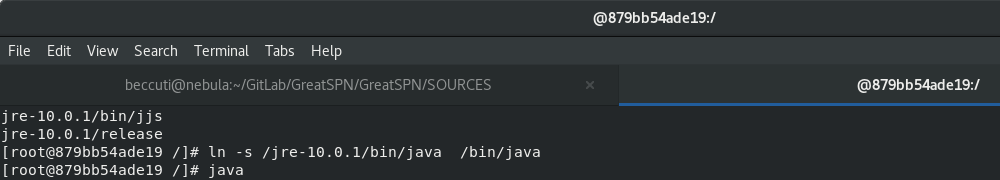
\includegraphics[width=0.95\columnwidth]{./Figure/javaFedora2}
  			\end{center}	
 \end{itemize}
}   	 
  
	\frame{
  \frametitle {Download and install FastQC}
  \begin{itemize} 		
  	\item Install \textbf{\color{NavyBlue} unzip} command using   \emph{\color{PineGreen} dnf install unzip.x86\_64};
          	\begin{center}
  			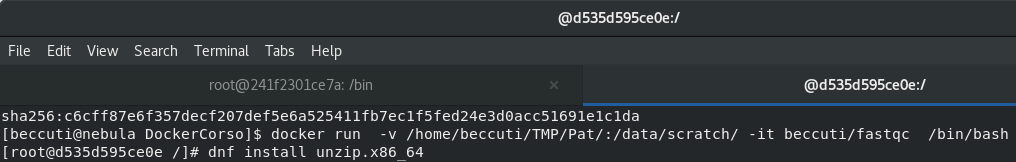
\includegraphics[width=0.95\columnwidth]{./Figure/unzipFedora}\vspace{0.2cm}
  			\end{center}		
  	\item Install  \textbf{\color{NavyBlue}perl} command using   \emph{\color{PineGreen} dnf install perl.x86\_64};
          	\begin{center}
  			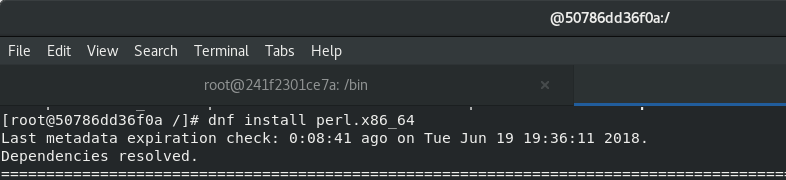
\includegraphics[width=0.95\columnwidth]{./Figure/perlFedora}\vspace{0.2cm}
  			\end{center}	
   \end{itemize}
} 			
  
  			
   
\frame{
  \frametitle {Download and install FastQC}
  \begin{itemize}  			
   \item Unzip  FastQC program;
   		    \begin{center}
  			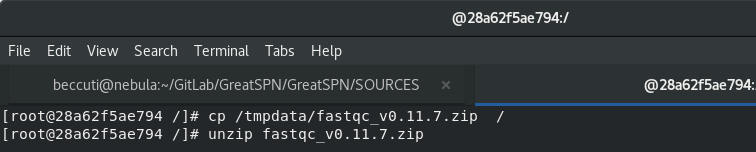
\includegraphics[width=0.95\columnwidth]{./Figure/fastqcFedora}
  			\end{center}	\vspace{0.1cm}
	\item Make FastQC program executable  and create a symbolic link in \emph{bin} for it;
	  	  		    \begin{center}
  			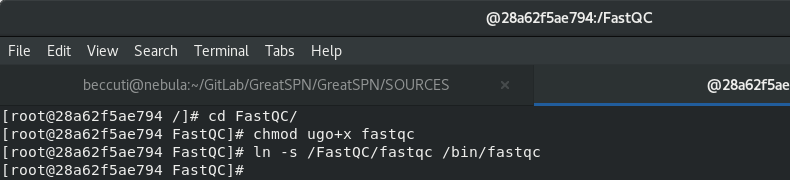
\includegraphics[width=0.95\columnwidth]{./Figure/fastqcFedora1}
  			\end{center}		\vspace{0.1cm}				
 \end{itemize}
}   	

\frame{
  \frametitle {Download and install FastQC}
  \begin{itemize}  			
 	\item Commit the updated image.
 	 	   \begin{center}
  			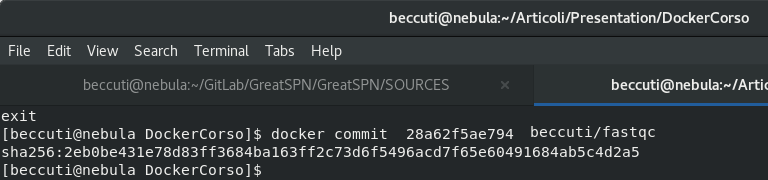
\includegraphics[width=0.95\columnwidth]{./Figure/fastqcFedora2}
  			\end{center}				
 \end{itemize}
}   	      
  	
 \frame{
  \frametitle { Download and install FastQC}
  \begin{itemize}  			
   \item  We use \textbf{\color{NavyBlue}gedit} to create our  bash script; \vspace{0.2cm}
   		    \begin{center}
  			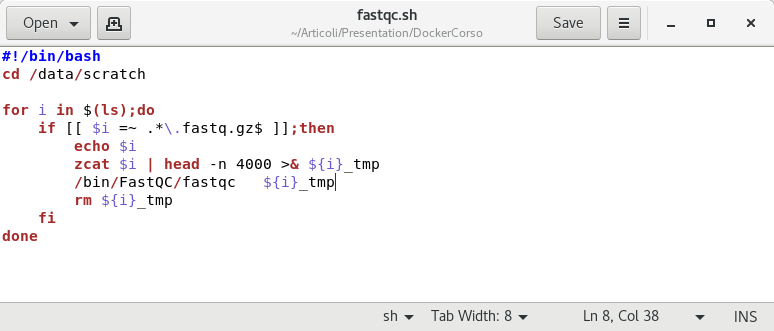
\includegraphics[width=0.95\columnwidth]{./Figure/fastqcGedit}
  			\end{center}	
  \end{itemize}
}   	    	  

 \frame{
  \frametitle { Download and install FastQC}
  \begin{itemize}   	  			
	\item Update the image adding the created script. \end{itemize}
	\vspace{0.2cm}
	  	  		    \begin{center}
  			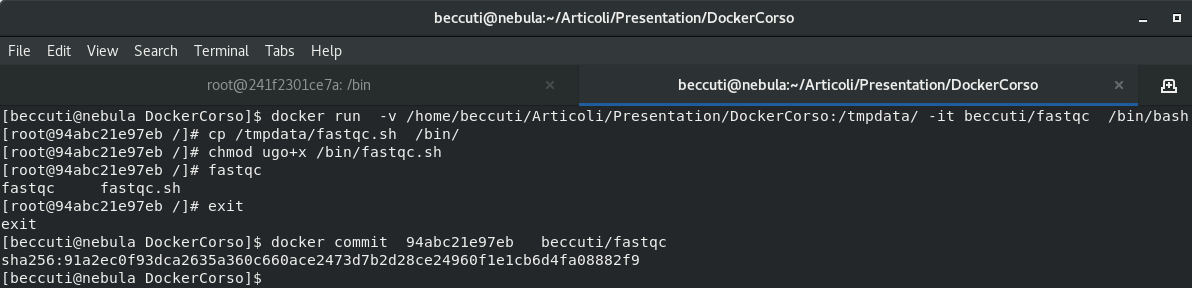
\includegraphics[width=1.0\columnwidth]{./Figure/fastqcshFedora}
  			\end{center}				

}  

 	    	  
 \frame{
  \frametitle {Run the embedded FastQC}
  \begin{itemize}   	  			
	\item Execute the embedded FastQC on .fastq files.\vspace{0.2cm}
	\item The folder containing .fastq files must be mount as /data/scratch  \end{itemize}
	
	  	    \begin{center}
  			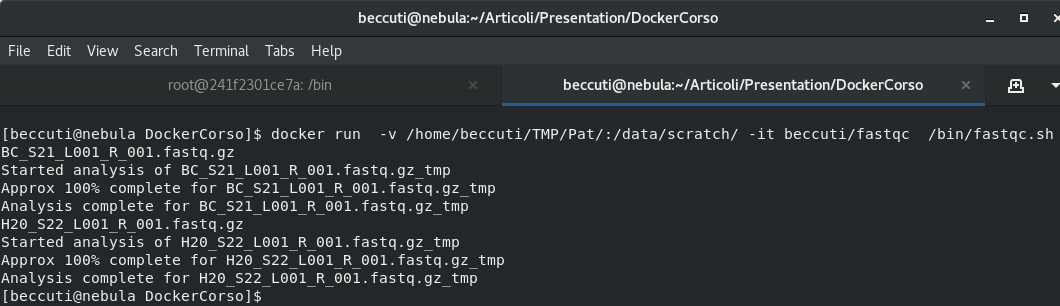
\includegraphics[width=1.0\columnwidth]{./Figure/fastqrunFedora}
  			\end{center}	
  						

}

 	    	  
 \frame{
  \frametitle {Run the embedded FastQC}
  \begin{itemize}   	  			
	\item FastQC output:
	  	    \begin{center}
  			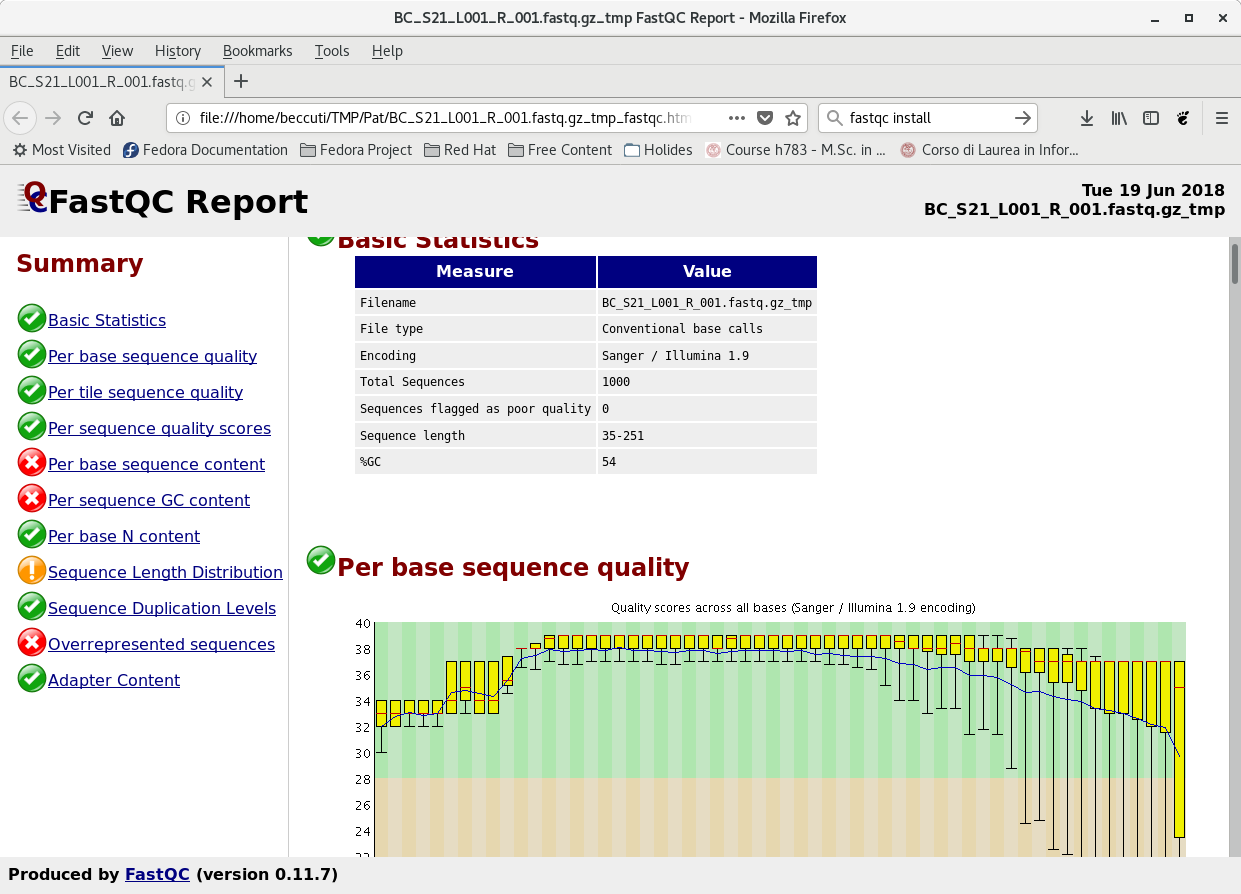
\includegraphics[width=0.78\columnwidth]{./Figure/fastqcHTML}
  			\end{center}	
  						
 \end{itemize}
}


   \frame{
  \frametitle {}
  \vspace{1.5cm}
  \centerline{\Huge \color{NavyBlue} \textbf{\emph{Create a docker image for }}}\vspace{0.05cm}
  \centerline{\Huge \color{NavyBlue} \textbf{\emph{FastQC tool using dockerfile}}}
  \vspace{0.4cm}
     	\begin{center}
  			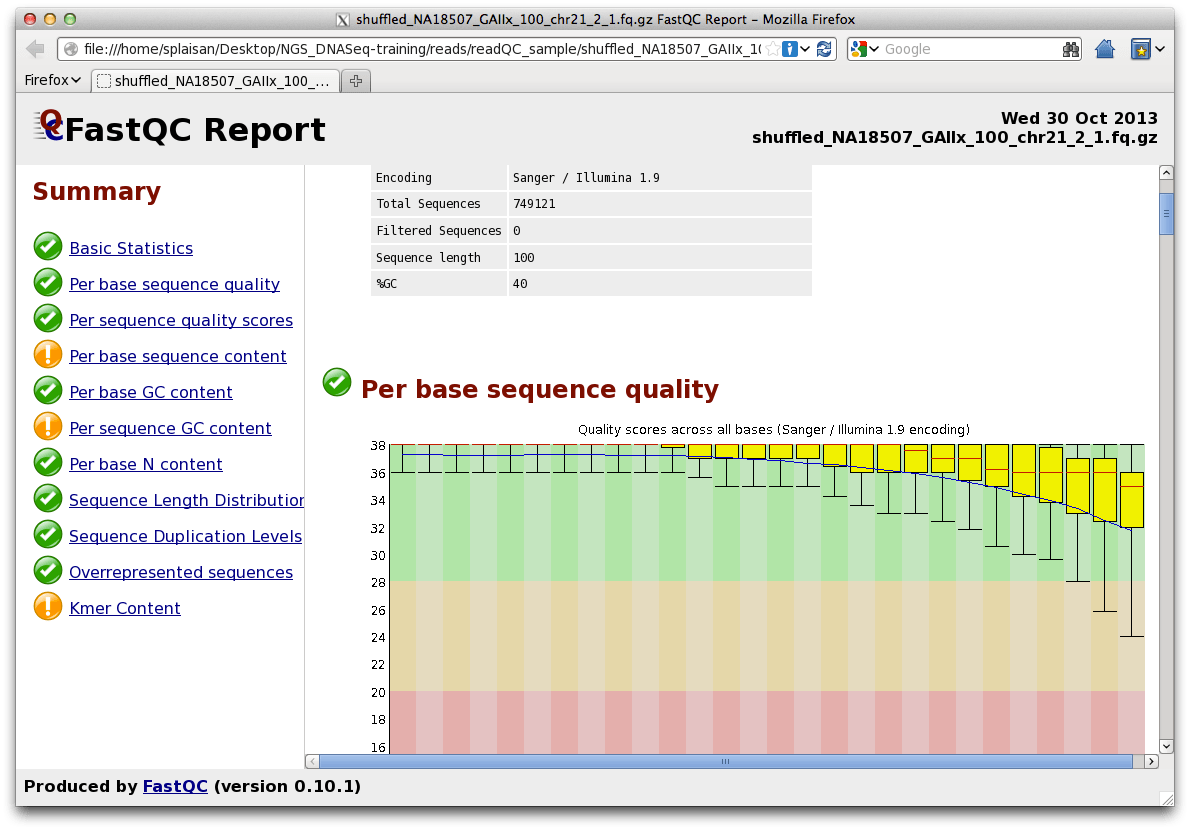
\includegraphics[width=0.60\columnwidth]{./Figure/FastQC}
  		\end{center} 

}


          \frame{
  \frametitle {Create a dockerfile}
  We use \textbf{\color{NavyBlue}gedit} to create our dockerfile; \vspace{0.2cm}
 \begin{center}
  			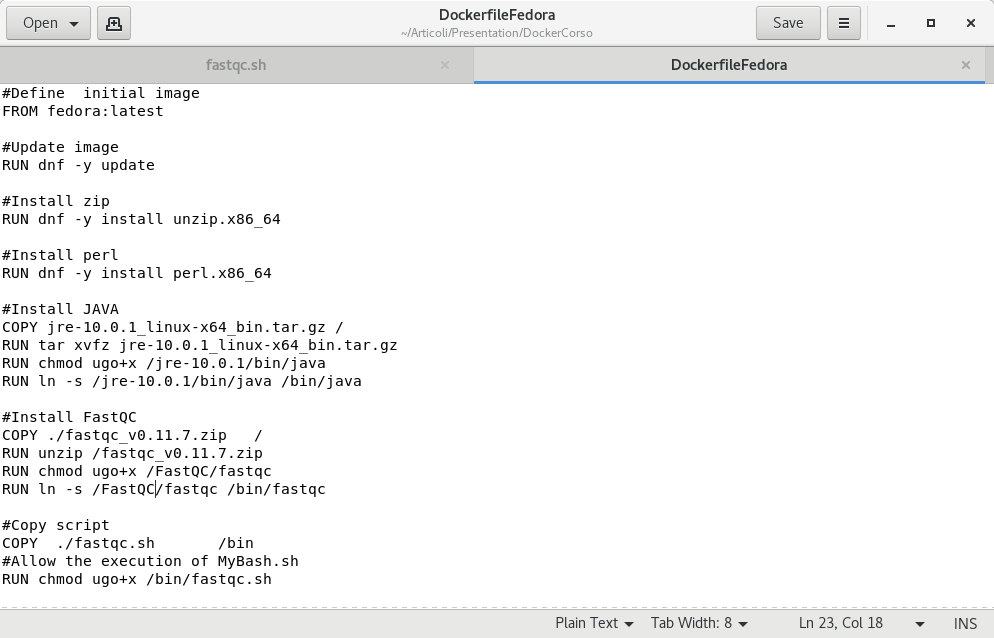
\includegraphics[width=0.95\columnwidth]{./Figure/gedit2}
 \end{center} 
  }

 \frame{
  \frametitle {Create FastQC image with dockerfile}
  
 \emph{\color{PineGreen} docker build -t  ``beccuti/fastqc2'' . -f DockerfileFedora} can be used to build an image from a Dockerfile.
     	\begin{center}
  			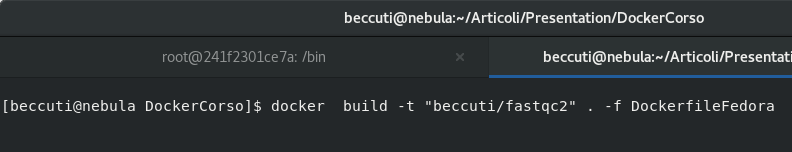
\includegraphics[width=1.00\columnwidth]{./Figure/build2}
  		\end{center}  
  		     	\begin{center}
  			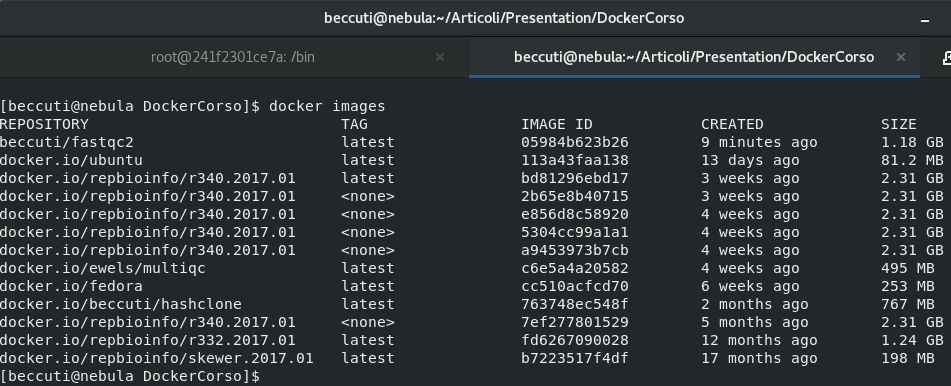
\includegraphics[width=1.00\columnwidth]{./Figure/build3}
  		\end{center}  
  
 } 	
  	